\section{Experimental evaluation}
\label{section:experiments}


\eat{
In Figure~\ref{fig:arch} we show the general view of the architecture.
and in Figure~\ref{fig:topo} we demonstrate the topology of the SOHO network, and in 
Figure~\ref{fig:prototype} we show working prototype.
}

\begin{figure}[!h]
        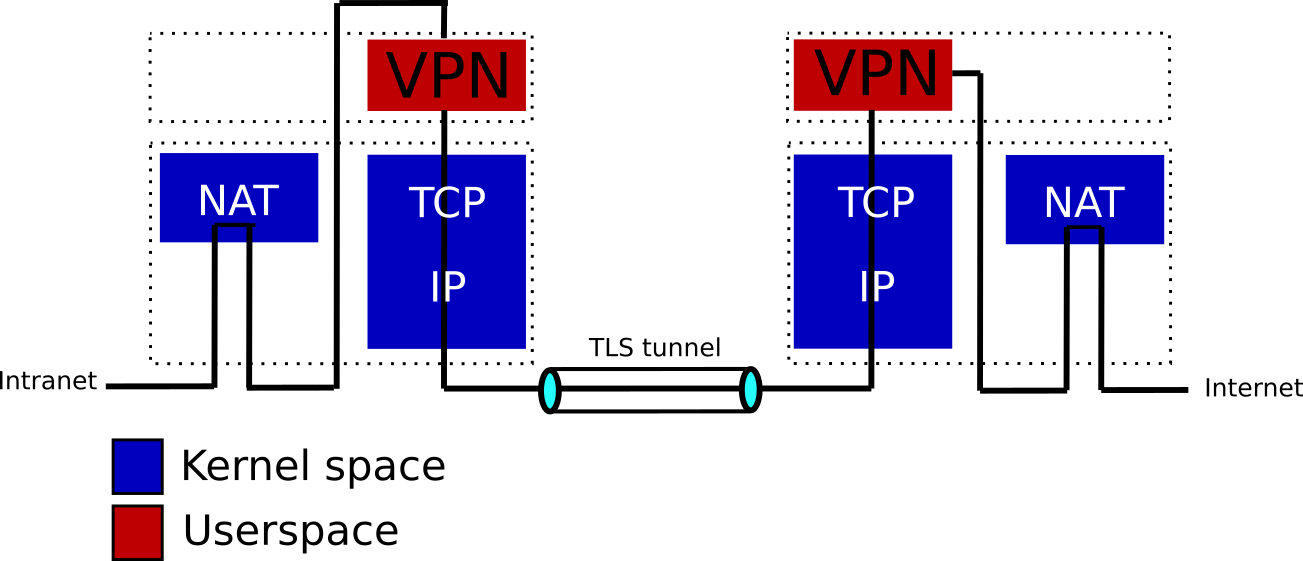
\includegraphics[width=0.5\textwidth]{graphics/architecture.png}
        \caption{Architecture of the prototype}
        \label{fig:arch}
\end{figure}

\eat{
\begin{figure}[!h]
        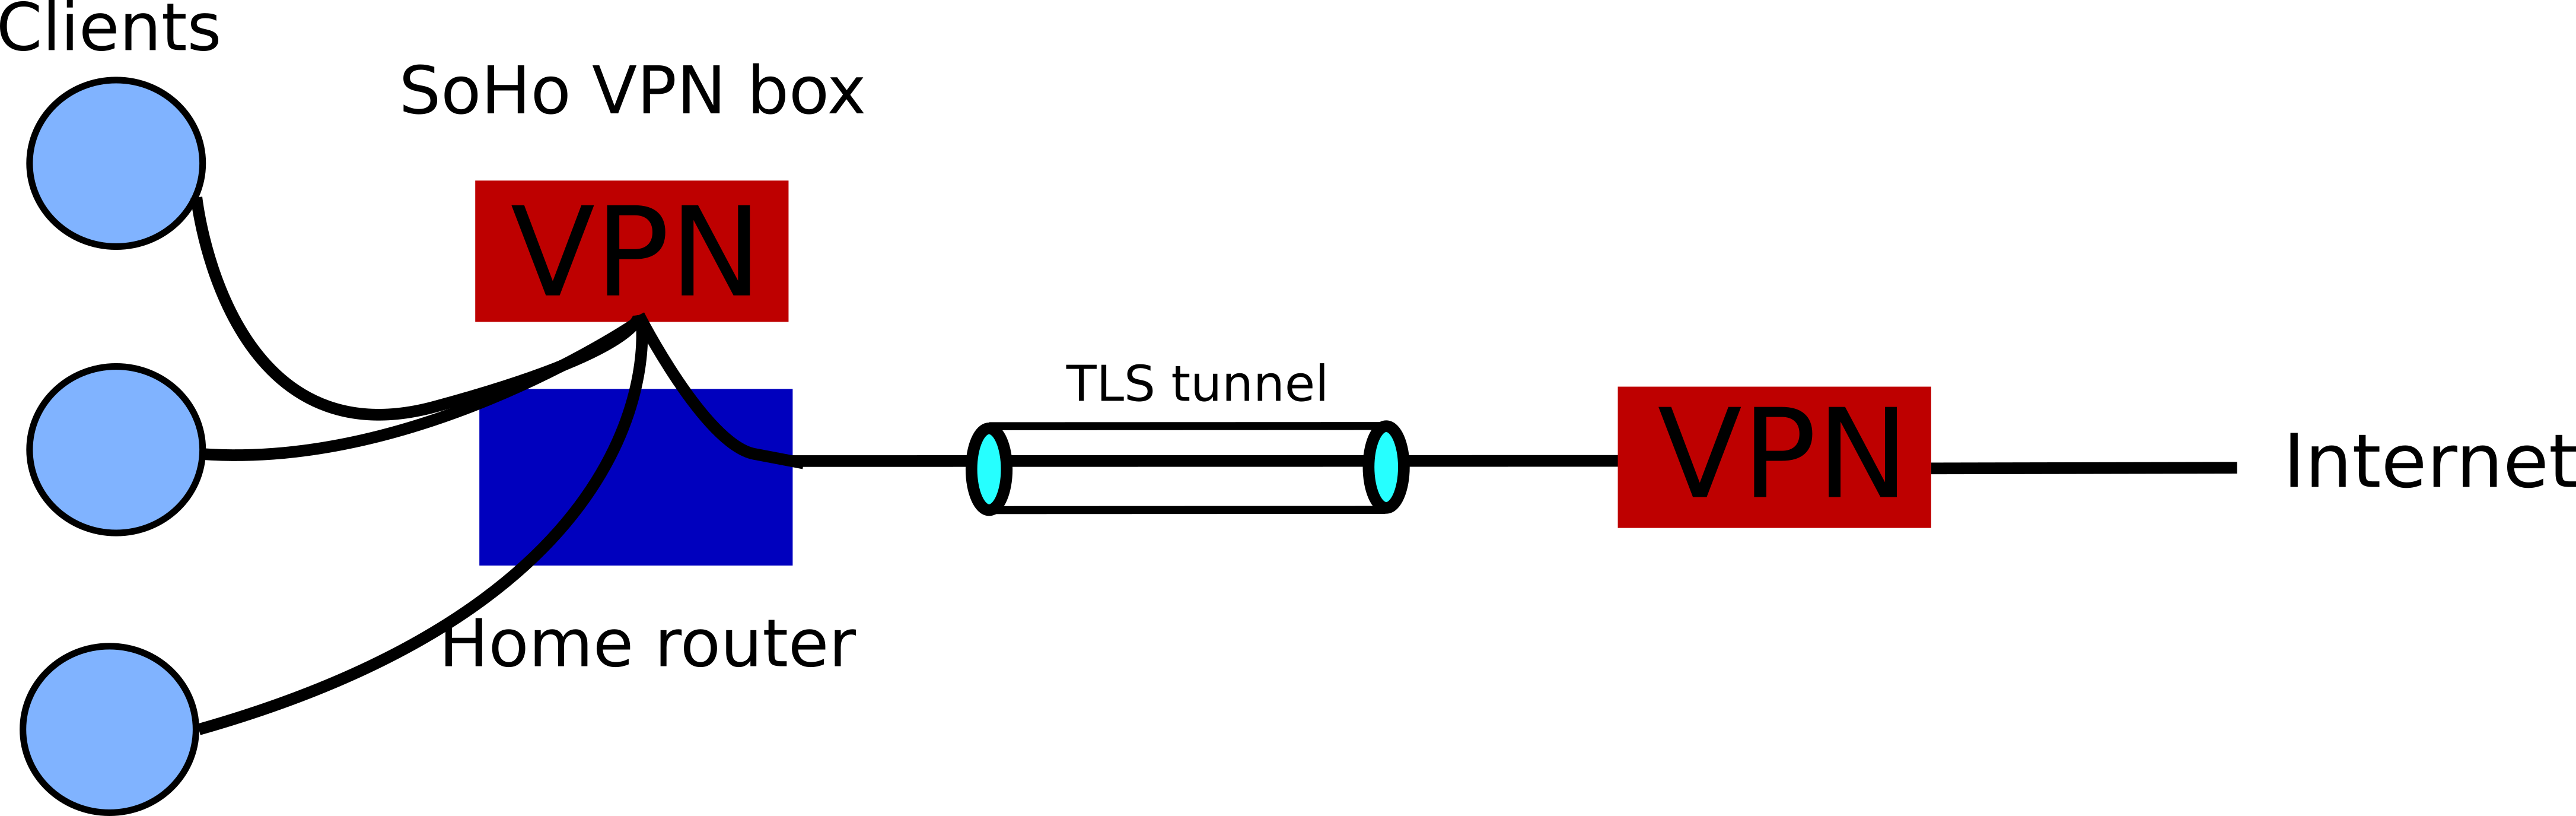
\includegraphics[width=0.5\textwidth]{graphics/topology.png}
        \caption{Topology of the SOHO network}
        \label{fig:topo}
\end{figure}
}

\eat{
\begin{figure}[!h]
        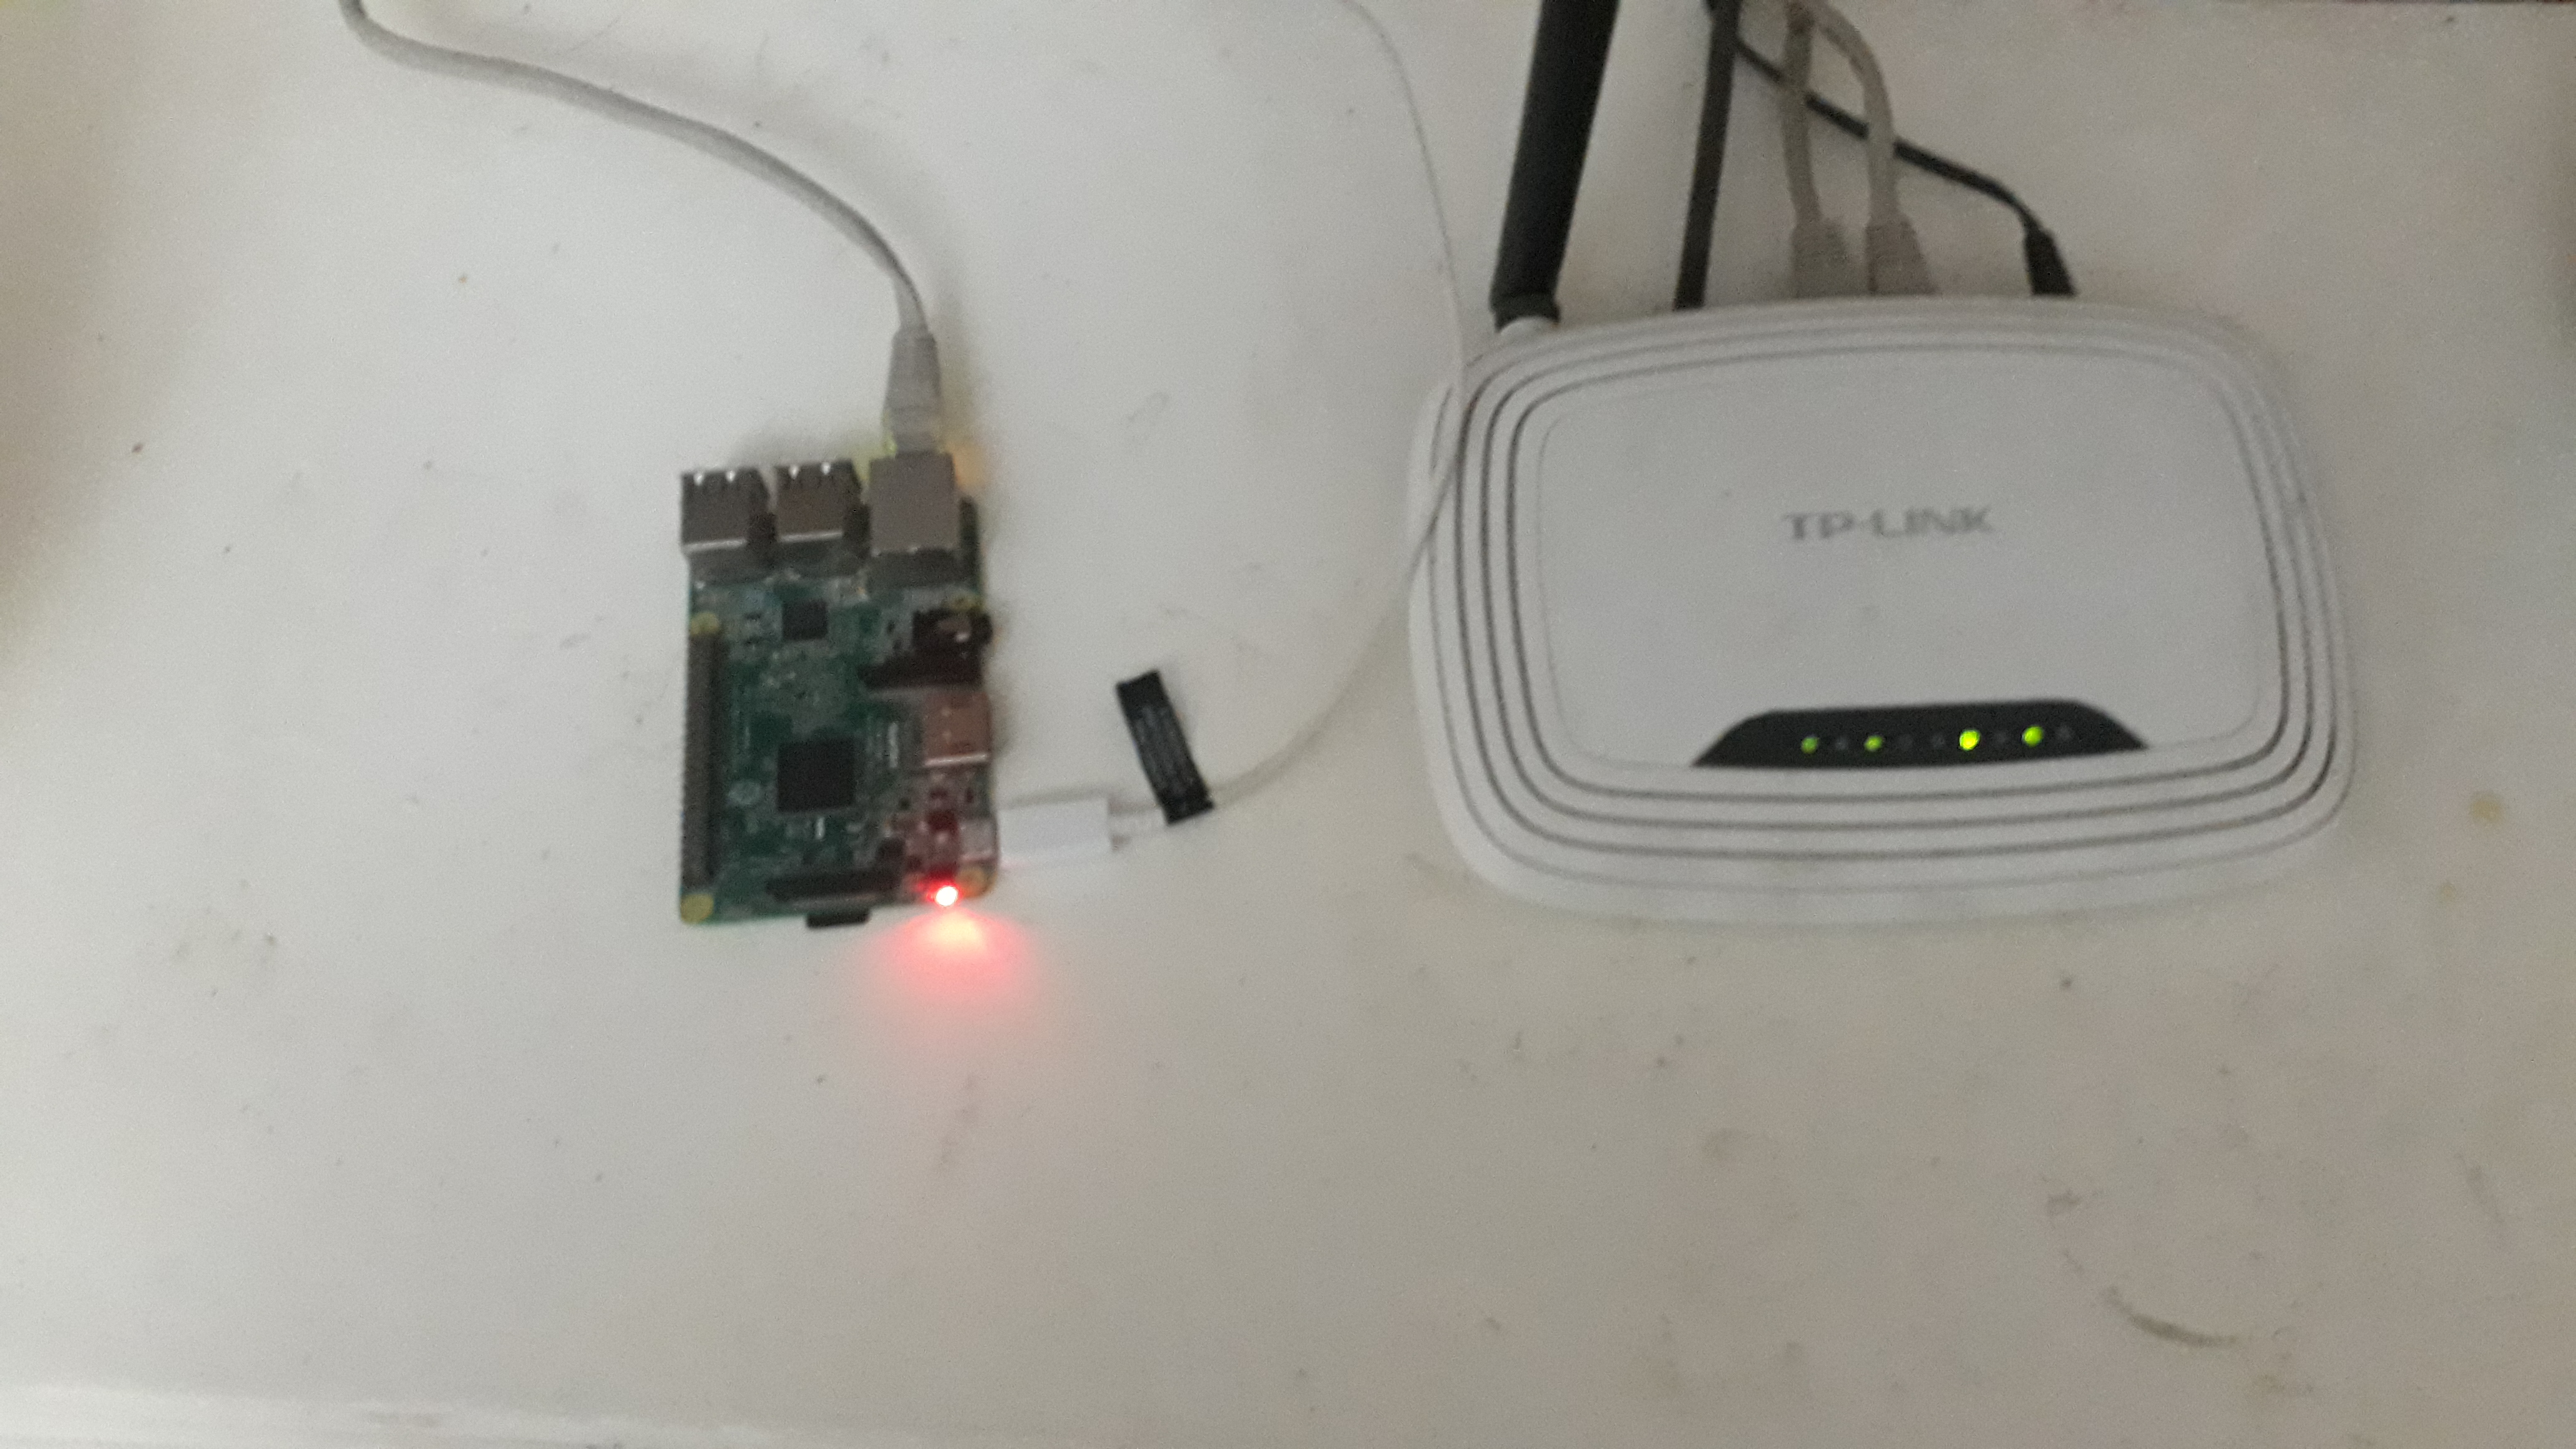
\includegraphics[width=0.5\textwidth]{graphics/prototype.jpg}
        \caption{Working prototype}
        \label{fig:prototype}
\end{figure}
}

In Figure~\ref{fig:arch} we show the general view of the architecture. 
We have made several experiments over the course of our work. The very first experiment was 
related to sending ping messages towards the VPN TLS server and observing the differences in
round trip times (basically, we have compared the round trip times between the setting in 
which tunnel was present and the setting in which the tunnel did not exist). Next, we have
sat down to measure the throughput between the local and remote machines. Basically, we have 
performed $50$ measurements for a setting, in which the traffic was going inside the tunnel
and the same number of measurements for the setting, in which the traffic was going 
normally (meaning, unencrypted and not encapsulated in TLS packets). To measure throughput,
we have used \texttt{wget} tool to download Linux kernel file from the Internet.

In Figure~\ref{fig:rtt} we show the distribution of round-trip times
(RTT). Mean RTT for VPN connection was $293.7$ ms, and mean RTT for 
plain ICMP was $103.3$ ms.

\begin{figure}[!h]
        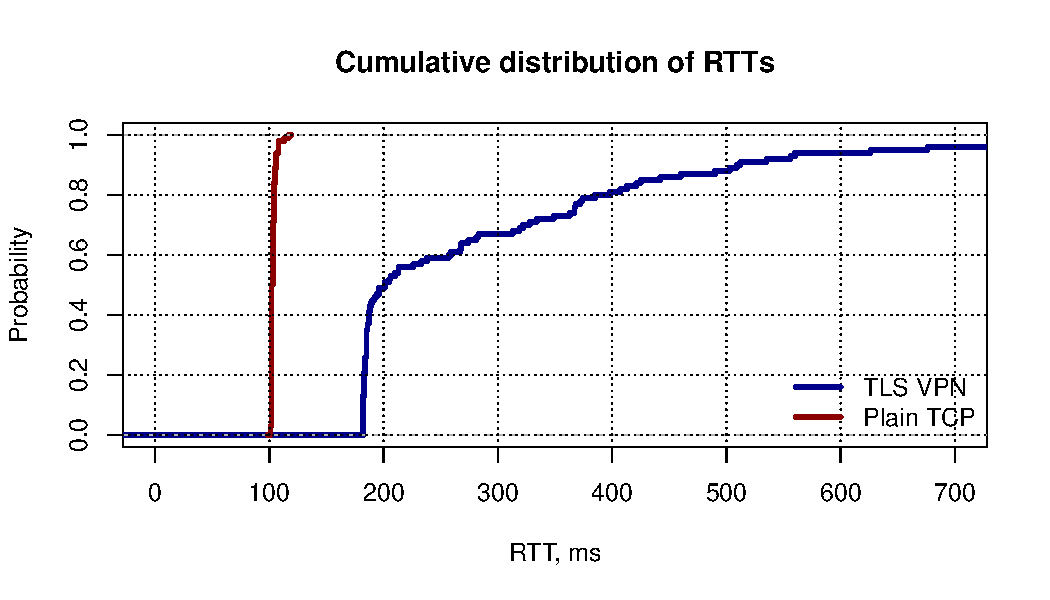
\includegraphics[width=0.5\textwidth]{graphics/rtt.pdf}
        \caption{Distribution of RTTs}
        \label{fig:rtt}
\end{figure}

In Figure~\ref{fig:iperf_distr} we show the distribution of the obtained throughput for both
TLS protected tunnel and regular TCP connections. Mean throughput value for the VPN connection was 
$608.7$ Kb/s, and mean throughput for plain TCP connection was $1890.4$ Kb/s. Given these results, we think that in this case the bottleneck is our implementation. However, we believe that our implementation of VPN tunnel is good enough for most small office settings.

\begin{figure}[!h]
        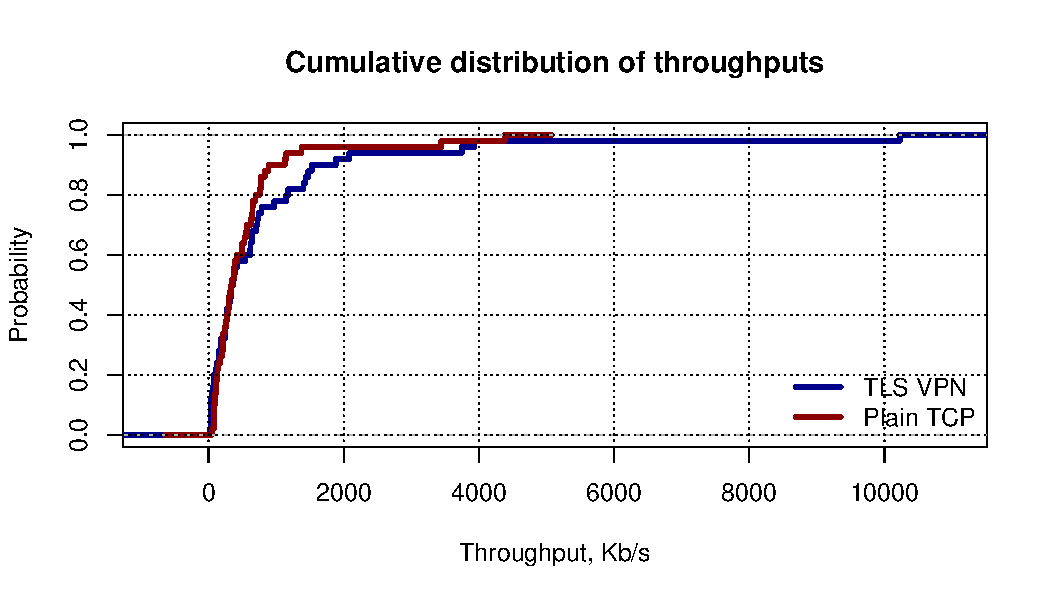
\includegraphics[width=0.5\textwidth]{graphics/throughput.pdf}
        \caption{Distribution of throughputs}
        \label{fig:iperf_distr}
\end{figure}

\eat{
Finally, we have made a successful experiment in which the tunnel was used for a long period of time
without interruption (the tunnel was used for several days).
}

\section{Future work}

Despite that the tunnel was running for several hours without interruption and we have implemented 
authentication layer, we still have seen several connection attempts, although unsuccessful, from the outside 
world. For the future, we plan to hide the VPN server behind the web server, so that only the users 
who know certain secret can access the VPN server. The idea is simple: when the user knocks by sending
HTTP GET request to a secret page, the web server opens a port and redirects the traffic from
the client to VPN server. Once the connection is established the server closes port. 